\documentclass[a4paper,12pt,english]{article}
\usepackage{babel}
\usepackage[]{graphicx}

%%%%%%%%%%%%%%%%%%%%%%%%%%%%%% LyX specific LaTeX commands.
%% Because html converters don't know tabularnewline
\providecommand{\tabularnewline}{\\}

%%%%%%%%%%%%%%%%%%%%%%%%%%%%%% Textclass specific LaTeX commands.
 \newenvironment{lyxcode}
   {\begin{list}{}{
     \setlength{\rightmargin}{\leftmargin}
     \setlength{\listparindent}{0pt}% needed for AMS classes
     \raggedright
     \setlength{\itemsep}{0pt}
     \setlength{\parsep}{0pt}
     \normalfont\ttfamily}%
    \item[]}
   {\end{list}}

 \newenvironment{lyxlist}[1]
   {\begin{list}{}
     {\settowidth{\labelwidth}{#1}
      \setlength{\leftmargin}{\labelwidth}
      \addtolength{\leftmargin}{\labelsep}
      \renewcommand{\makelabel}[1]{##1\hfil}}}
   {\end{list}}

\begin{document}

\title{Specification of the PFS File Format\\version 1.5}

\maketitle

\section{Introduction}

This document contains a detailed specification of the pfs file
format. PFS file format is intended to store in particular
high-dynamic range images, but it is also flexible enough to store
additional data, like depth map or motion flow. To learn how PFS
format can be useful and why it is different from existing image
formats, see a list of Frequently Asked Questions of the PFS tools
package. Information in this section should be sufficient to implement
pfs compatible reader or writer.

\section{Copyright}

Copyright (c)  2003  Rafal Mantiuk and Grzegorz Krawczyk

Permission is granted to copy, distribute and/or modify this document
under the terms of the GNU Free Documentation License, Version 1.2 or
any later version published by the Free Software Foundation; with no
Invariant Sections, no Front-Cover Texts, and no Back-Cover Texts.  A
copy of the license is included in the section entitled "GNU Free
Documentation License".

\section{Change History}

\begin{itemize}
\item 1.0 (15.12.2004 RM) --- Original version
\item 1.1 (14.02.2005 RM) --- Colon ':' is no longer allowed in the name of a tag; Added a conceptual UML data-model
\item 1.2 (16.03.2006 RM) --- Fixed typos (thanks to grendelkhan)
\item 1.3 (16.08.2006 RM) --- Added a list of registered channel names; added comments on endianness)
\item 1.4 (28.06.2007 RM) --- Fixed column-/row-major ambiguity (thanks to Matt)
\item 1.5 (06.08.2007 RM) --- Specified maximum string lengths and valid value ranges. Added suggestion to prepend custom channel names with ''x''. (thanks to Martin)
\item 1.6 (03.10.2008 RM) --- Added a new tag 'BITDEPTH'
\end{itemize}


\section{General Structure}

A pfs-stream is a byte-stream that contains one or more frames. Each
frame is stored in the pfs-stream right after another frame, without
any markers or separators between them. End of file indicates that
there are no more frames in the pfs-stream.

A conceptual data model of the pfs stream is shown in
Figure~\ref{cap:data-model}. A pfs-stream can contain any number of
frames, which include any number of channels. Both frame and channel
has an associated tag-container, which can contain any number of tags
(name=value pairs).

\begin{figure}
  \centering 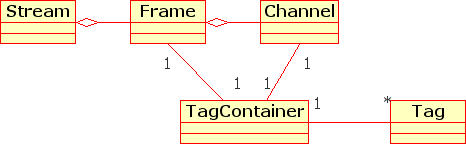
\includegraphics[width=\textwidth]{data_model.png}
\caption{A conceptual UML data model of the pfs-stream}
\label{cap:data-model}
\end{figure}


A structure of a single frame is shown in Table~\ref{cap:pfs-frame}.
A frame encoded in the pfs format consists of a text header followed
by binary data. The header contains information on frame size, number
of channels and tags. Data items in the header are separated by end of
line (EOL) characters.  Note that only a unix-type EOL character is
allowed (a single character of the ASCII code 10).  MSDOS-type EOL is
not allowed. To avoid portability problems, use C string
``{\tt\textbackslash{}x0a}'' instead of ``{\tt\textbackslash{}n}''.
Note that the header ends with a {\tt ENDH} string, which is not
followed by an EOL character. This prevents C formated IO functions,
like {\tt fscanf}, from reading both the EOL character and first bytes of
binary data that happen to have the values of white spaces.

The binary data part of a frame follows text header and holds a 2D
array of floating points for each channel. The structure of a channel
is described in the next section.
%
\begin{table}
\begin{tabular}{|l|l|p{5cm}|}
\hline 
Data&
Type&
Description\tabularnewline
\hline
\hline 
\textbf{PFS1\P}&
&
Constant identifier\tabularnewline
\hline 
width height\P&
\emph{int int}&
Width and height of each channel (1--65535) \tabularnewline
\hline 
channelCount\P&
\emph{int}&
Number of channels (1--1024)\tabularnewline
\hline 
frameTagCount\P&
\emph{int}&
Number of tags associated with the frame (0--1024)\tabularnewline
\hline
\emph{for i=1:frameTagCount}&
&
\tabularnewline
\hline
~~tagName\textbf{=}tagValue\P&
\emph{string string}&
An i-th tag: name=value pair (max length of \texttt{strcat(string, string)} - 1023)\tabularnewline
\hline
\emph{for i=1:channelCount}&
&
\tabularnewline
\hline
~~channelName\P&
\emph{string}&
Name of the i-th channel (max string length -- 32)\tabularnewline
\hline
~~channelTagCount\P&
\emph{int}&
Number of tags associated with i-th channel (0--1024)\tabularnewline
\hline
~~\emph{for j=1:channelTagCount}&
&
\tabularnewline
\hline
~~~~tagName\textbf{=}tagValue\P&
\emph{string string}&
An i-th tag: name=value pair (max length of \texttt{strcat(string, string)} - 1023)\tabularnewline
\hline
\textbf{ENDH}&
&
Signalizes the end of the header\tabularnewline
\hline
\emph{for i=1:channelCount}&
&
\tabularnewline
\hline
~~channelData&
\emph{bin-float}{[}w{]}{[}h{]}&
Row-major array of 32-bit floating points\tabularnewline
\hline
\end{tabular}


\caption{\label{cap:pfs-frame}A structure of pfs-frame. Bold font denotes
  literal strings. '\P'~is a unix-type end of line character
  (ASCII code 10). Types: \emph{int} -- integer value given as string;
  \emph{string} -- a string of one or more characters (1-byte ASCII); \emph{bin-float}{[}w{]}{[}h{]}
  -- a row major array of 32-bit floating point numbers in binary format. The range of valid values and maximum string lengths are given in the parenthesis in the ``description'' column.}
\end{table}

\section{Channels}

Channels are two-dimensional arrays of floating point numbers, which
can contain anything from color data to motion flow and depth (z-buffer)
information.  Channels are written in a stream in the same order as they
are listed in the header. Note that no assumption can be made on the
order of channels --- it may differ from file to file and some
applications may even reverse that order.

For the sake of performance, channel data are encoded in binary
format. Each cell (pixel) of an array should be encoded as a IEEE
Standard 754 Floating Point Number. Fortunately, this representation
is used by CPU for most architectures, including Intel-based PC's, so
it is enough to store the values in memory as a C 'float' type and
then write them to an IO stream. An array should be encoded in a
stream in a row major order --- all cells of the first row are
followed by the cells of the second row and so on. The encoding starts
from the top left corner. The bytes should be encoded in the
little-endian order (LSB), which is appropriate for the x86
platform\footnote{Current implementation of the pfs library does not
  handle big-endian system, so the pfs files generated on x86 and
  powerPC platforms are not compatible}.

This version of the pfs format specification defines the following
channels:
\begin{description}
  \item {\bf X} --- X color component of the CIE XYZ color space. See comments below.
  \item {\bf Y} --- Y color component of the CIE XYZ color space. See comments below.
  \item {\bf Z} --- Z color component of the CIE XYZ color space. See comments below.
  \item {\bf DEPTH} --- Depth channel. Format of the depth information is currently not standardized.
  \item {\bf ALPHA} --- Alpha channel that encodes transparency. The values should be in the range from 0 to 1.
\end{description}
If other information than color, depth and alpha needs to be stored in
a channel, a custom name starting with a lower-case ''x'' letter
should be used. If you think that a particular channel name should be
registered in this document, feel free to suggest it on the {\tt pfstools@googlegroups.com} 
discussion group.

Color information must be represented in CIE XYZ ($2^\circ$ standard
observer) color space. Depending on the value of the LUMINANCE tag,
color data are linear (RELATIVE -- linearly related to luminance),
linear and calibrated (ABSOLUTE -- the values of Y channel represent
luminance in $cd/m^2$), or non-linear (DISPLAY -- gamma-corrected).
The preferred representation is a 'linear and calibrated'.
'non-linear' is only a temporary representation used before data is
written to low dynamic range image files (PNG, JPG) or displayed. For
more information refer to the next section --- \ref{sec:tags}. The
channels must be named using upper case letters: 'X', 'Y' and 'Z'. For
color images, all three X, Y and Z channels must be given. It is
enough to include 'Y' channel for gray-level images.


\section{Tags}
\label{sec:tags}

pfs format allows for storing tags, which are 'name=value' pairs. Tags
are robust mechanism for specifying additional information within a
pfs-stream. Both the name and value should be a text string, i.e. if a
floating point number is to be stored, it should be converted into a
text string. The name must not contain '=' and ':' character (some
programs use notation 'channel\_name:tag\_name' to assign a tag to the
channel). Spaces in front of and after '=' are allowed, although they
will not be skipped and they will be interpreted as a part of name or
value strings. Tags can be associated with a frame or separate
channel, depending how they are placed in the text header of the pfs
frame (see Table~\ref{cap:pfs-frame}).  Each tag associated with a
single frame or channel must have an unique name. There is no limit to
the number of tags.

In general, tags can be used to store any user defined data, but there
are also several tags that are reserved and are part of the pfs
format. Those tags let precisely define content of the pfs stream.
The reserved tags are listed below:

 \begin{description}
 \item LUMINANCE specifies a photometric content of the XYZ color
   channels or Y luminance channel alone. LUMINANCE tag distinguishes
   between different methods of storing lumiance data. This tag must
   be associated with a frame and the frame must contain either all
   XYZ channels or Y channel. Possible values are: ABSOLUTE, RELATIVE,
   and DISPLAY.
   \begin{description}
   \item ABSOLUTE Set the LUMINANCE tag to this value if the high-dynamic
     range data is calibrated. Y channel should contain absolute
     luminance values given in $cd/m^2$. Note that luminance values
     must be $\geq0$ for calibrated content.
   \item RELATIVE High-dynamic range data is of RELATIVE LUMINANCE if
     it is not calibrated, that is Y channel data is proportional
     to luminance, but nothing is known about absolute value of
     luminance. This is the case of most of the high-dynamic range
     images available on Internet. 
   \item DISPLAY If the data comes from low-dynamic range file and no
     colorimetric information is provided in ICC profile, the data is
     simply given in pixel values of an unknown display device. This
     is the worst case, but also most common as most of the
     low-dynamic range formats (jpeg, png, tiff) do not contain any
     data that can be used to recover luminance values. The values of the Y
     channel can range from $0$ to $1$ and are already gamma
     corrected.
   \end{description}
   If the LUMINANCE tag is not specified in the pfs-stream, RELATIVE is assumed.

   Example: LUMINANCE=ABSOLUTE
   
 \item VISUAL\_CONTENT tag specifies visual content of the XYZ color
   channels or Y luminance channel alone. If an image was captured as
   high-dynamic range photograph, it has one-to-one correspondence
   with the real word, therefore its VISUAL\_CONTENT is MEASUREMENT.
   However, if the same image has been tone mapped (or gamut mapped)
   it still resembles appearance of the real word scene, but it has no
   longer one-to-one correspondence. In this case its VISUAL\_CONTENT
   is RENDERING.  This tag is typically set to rendering after tone
   mapping of high-dynamic range images. This tag must be associated
   with a frame and the frame must contain either all XYZ channels or
   Y channel.
   \begin{description}
   \item MEASUREMENT Set VISUAL\_CONTENT tag to MEASUREMENT if the
     image has one-to-one correspondence with the real word, i.e. it
     contains measured data.
   \item RENDERING Set VISUAL\_CONTENT to RENDERING if the image has the same
     appearance as the real world scene, but there is no photometric
     correspondence.
   \end{description}
   If the tag is not specified in the pfs-stream, MEASUREMENT is assumed.
   If LUMINANCE tag is set to DISPLAY, the VISUAL\_CONTENT is assumed to be
   RENDERING.

   Example: VISUAL\_CONTENT=RENDERING
   
 \item WHITE\_Y defines the value of channel Y that is perceived as
   reference white. The value should be given in units of an Y
   channel.  If LUMINANCE=ABSOLUTE, the white point is given in
   $cd/m^2$. The value of this tag should be a single floating point
   number in a text format.

   Example: WHITE\_Y=100
   
 \item WHITE\_x, WHITE\_y tags define relative coordinates of color
   that is perceived as reference white. The value of those tags must
   be a floating point number in a text format. The value is given
   as a relative colorimatric coordinates of the CIE XYZ space ($2^\circ$
   standard observer) $y=Y/(X+Y+Z)$ and $x=X/(X+Y+Z)$.

   If the tag is not specified, D65 white point is assumed: $x=0.3127\:y=0.3290$

   Example: WHITE\_x=0.3457~~WHITE\_y=0.3585

 \item FILE\_NAME contains a string with the name of a source file.
   This can be used to locate the origin of a frame.

   Example: FILE\_NAME=my\_sequence\_frame\_0000.hdr

 \item BITDEPTH specifies the number of bits, that are required to
   store a single channel in a display-referred image
   (LUMINANCE=DISPLAY) without quality loss. The number should be from
   1 to 32. 

   Example: BITDEPTH=16

 \end{description}
 
\section{Discussion}

The structure of pfs files is a compromise between simplicity and
robustness and (as well) between portability and performance. Therefore
a small header is stored in text format as this is the easiest to
decode on different platforms. Storing image data as text would result
in too much overhead and thus binary format is used. Since parsing a file
is typically more difficult to implement than writing it, pfs format
tries to make parsing files as easy as possible. This is why sizes of
all variable length structures are given first and then actual data
follows.
\end{document}
